\chapter{Scalar Field Theory}

In this chapter, we study the interacting scalar field theory
\begin{equation}
\begin{aligned}
	\mathcal L &= \mathcal L_0 + \mathcal L_{\mathrm{int}}, \\
	\mathcal L_0 &=\frac{1}{2}\partial^\mu \phi \partial_\mu \phi -\frac{m^2}{2}\phi^2, \\
	\mathcal L_{\mathrm{int}} &= -\frac{g}{4!}\phi^4.
\end{aligned}
\end{equation}
As we have discussed, because of the interaction, the field and coefficients will be renormalized:
\begin{equation}
\begin{aligned}
	\phi &= \sqrt{Z_\phi} \phi_R, \\
	m &= \sqrt{Z_m} m_R, \\
	g &= Z_g g_R.
\end{aligned}
\end{equation}
The renormalized Lagrangian becomes:
\begin{equation}
	\mathcal{L}
	= Z_\phi \frac{1}{2} (\square\phi_R)^2 - Z_m Z_\phi \frac{m_R^2}{2} \phi_R^2 - Z_g Z_\phi^2 \frac{g_R}{4!}\phi_R^4.
\end{equation}
We can formally divided the renormalized theory into three parts: free theory part, interaction part, and the counter terms:
\begin{equation}
\begin{aligned}
	\mathcal L &= \mathcal L_0 + \mathcal L_{\mathrm{int}} + \mathcal L_{\mathrm{ct}}, \\
	\mathcal L_0 &= \frac{1}{2} (\square\phi_R)^2 - \frac{ m_R^2}{2} \phi_R^2, \\
	\mathcal L_{\mathrm{int}} &= -\frac{g_R}{4}\phi_R^4, \\
	\mathcal L_{\mathrm{ct}} &= A \frac{1}{2} (\square\phi_R)^2 - B\frac{ m_R^2}{2} \phi_R^2 - C \frac{g_R}{4!} \phi_R^4,
\end{aligned}
\end{equation}
where the coefficients in the counter terms are:
\begin{equation}
	A = Z_\phi-1, \quad 
	B = Z_m Z_\phi - 1, \quad 
	C = Z_g Z_\phi^2 - 1.
\end{equation}
The counter terms come from the renormalization factors, which can be formally infinity but are perturbatively of order $O(g)$, and thus are regarded as additional perturbations to the free theory.




\section{Perturbative Renormalization}

\subsection{First-order Correction to the Propagator}
Consider the first order perturbation to the propagator:
\begin{equation}
\begin{aligned}
	i \Delta^{(1)}(k)
	&= 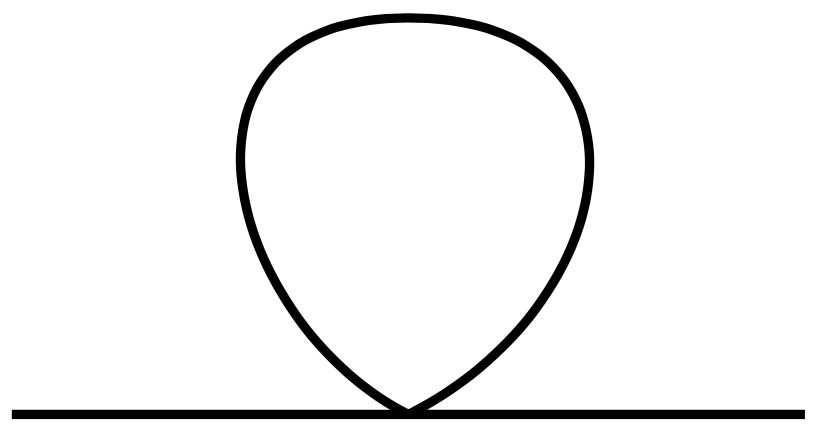
\includegraphics[align=c, width=0.4\linewidth]{pics/KG-3.png} \\
	&= i\Delta_0(k) \left[-\frac{g}{2}\int \frac{d^4 q}{(2\pi)^4} \frac{1}{q^2-m_R^2} + i(Ak^2-Bm_R^2) \right] i\Delta_0(k).
\end{aligned}
\end{equation}
Note that in the loop diagram, there is in total ($4 \times 3 = 12$) identical diagrams, and so gives the coefficients.
A simpler counter rule is that if the diagram has no symmetry, there is in total $4!$ identical diagrams and the denominator cancels out exactly, while for any remaining symmetries, the symmetry factor will remain in the denominator.
For the loop diagram we considered here, the symmetry factor is $2$.

Note that the second order correction to the Green's function has one ``ingoing'' leg and one ``outgoing'' leg, the core (or the amputated Green's function) in this case is called the \textit{self-energy} $i\Sigma(k^2)$:
\begin{equation}
	i\Sigma(k^2) = -\frac{g}{2}\int \frac{d^4 q}{(2\pi)^4} \frac{1}{q^4-m_R^2} + i(Ak^2-Bm_R^2).
\end{equation}
The integral is divergent, that when the counter terms come to rescue.
The divergent part of the integral can be absorbed into the coefficients, or be canceled by the counter terms.
In the following, we will see that the divergent integral
\begin{equation}
	I \equiv -\frac{g}{2} \int \frac{d^4 q}{(2\pi)^4} \frac{1}{q^4-m_R^2}
\end{equation}
can be regularized.
The regularization is typically controlled by a parameter which will recover the infinity when taking a specific limit.
The physical observable shall not depend explicitly on the regularization parameter, so the final result is free from divergent even if we take the limit.


\subsubsection{Regularization of the Divergent Integral}
Consider the integral
\begin{equation}
	I = -\frac{g}{2} \int\frac{d \omega}{2\pi} \int\frac{d^3 q}{(2\pi)^3} \frac{1}{\omega^2 - \bm q^2-m_R^2 -i\epsilon}
\end{equation}
Since the singularity locates at $\pm(\sqrt{\bm q^2+m_R^2}-i\epsilon)$, we can analytically change the integral of $\omega$ from real axis to the imaginary axis anti-clock-wisely, the result is equivalent to the substitution $\omega \rightarrow i\omega$.
The new integral is defined on the 4D Euclidean space:
\begin{equation}
\begin{aligned}
	I &= i \frac{g}{2} \int \frac{d^4 q}{(2\pi)^4} \frac{1}{q^2 + m_R^2} \\
	&= i\frac{g}{2} \frac{\Omega_4}{(2\pi)^4} \int_0^\infty dq \ \frac{q^3}{q^2 + m^2_R},
\end{aligned}
\end{equation}
where 
\begin{equation}
	\Omega_d = \frac{2 \pi^{\frac{d}{2}}}{\Gamma\left(\frac{d}{2}\right)}
\end{equation}
is the $d$-dimensional spherical area.

Till now the integral is essentially the same and thus still divergent.
Now we are going to regularize the expression.
One most frequently used regularization scheme is the \textit{dimensional regularization}.
It take note of the fact that the divergence of the integral only happens at integer dimension.
When we put the field theory to ($d=4-\varepsilon$)-dimensional space, the integral becomes:
\begin{equation}
	I_\varepsilon = i\frac{g\tilde{\mu}^\varepsilon}{2}\frac{\Omega_{4-\varepsilon}}{(2\pi)^{4-\varepsilon}} \int_0^\infty dq\ \frac{q^{3-\varepsilon}}{q^2+m_R^2}.
\end{equation}
Note that we have introduced a mass scale $\tilde\mu$ to get the correct dimensionality.
The integral is now convergent.
The specific form the the integral is not important, but we are concerned about the expansion near $\varepsilon = 0$. 
All the computation here can be done automatically (in \texttt{Mathematica}), and the result is
\begin{equation}
\begin{aligned}
	I_\varepsilon &= i\frac{g m_R^2}{32\pi^2} \left[\frac{2}{\varepsilon}+1+\log \left(\frac{4 \pi \tilde{\mu}^2 e^{-\gamma_E}}{m_R^2}\right)\right] + O(\varepsilon) \\
	&\equiv i\frac{g m_R^2}{32\pi^2} \left[\frac{2}{\varepsilon}+1+\log \left(\frac{\mu^2}{m_R^2}\right)\right] + O(\varepsilon),
\end{aligned}
\end{equation}
where $\gamma_E$ is the Euler constant. 
We have seen that the integral is controlled by the parameter $\varepsilon$.
In the $\varepsilon \rightarrow 0$ limit, the integral is divergent.


\subsubsection{Renormalization Using the Counter Terms}
We are now going to renormalize the theory.
Note that in the self-energy definition
\begin{equation}
	\Sigma(k^2) = \frac{1}{i} I + A k^2-B^2 m_R^2,
\end{equation}
we have the freedom to choose the counter terms that cancel the infinity.
To the first order, the coefficients can be
\begin{equation}
	A = O(g^2), \quad
	B = \frac{g}{16\pi^2 \varepsilon} + O(g^2).
\end{equation}
The result is
\begin{equation}
	\Sigma(k^2) = \frac{g m_R^2}{16\pi^2} \log \left(\frac{\mu}{m_R}\right)
	+\frac{g m_R^2}{32\pi^2}+O(\varepsilon).
\end{equation}
The one-loop correction also leads to a infinite \textit{Dyson series}:
\begin{equation}
\begin{aligned}
	i\Delta(k) &= i\Delta_0(k) + i\Delta_0(k)\sum_{n=1}^\infty \left[i\Sigma(k^2)i\Delta_0(k)\right] \\
	&= \frac{i}{k^2 -m_R^2 + \Sigma(k^2)}.
\end{aligned}
\end{equation}



\subsubsection{Physical Observables}
The physical observable here is the rest mass $m_0$, which is experimentally measurable.
It equals to the pole of the propagator, i.e.,
\begin{equation}
	m_R^2 - \Sigma(m_0^2) = m_0^2.
\end{equation}
Depending on the mass scale $\mu$ we choose, the renormalized mass $m_R$ may or may not equal to the rest mass.
Specifically, we can choose mass scale so that $m_R = m_0$, that is
\begin{equation}
	\Sigma(m_0^2) = 0 \quad \Longrightarrow \quad
	\mu = e^{-\frac{1}{2}} m_0.
\end{equation}
To the first order, the self-energy has no momentum dependence, so there is no physical prediction.




\subsection{Second-order Correction to the Vertex}

Now consider the second order correction to the vertex function, which is the connected, amputated 4-point Green's function.
The perturbation correspond to 3 different Feynman diagrams together with a vertex counter term.
The explicit form is: 
\begin{equation}
\begin{aligned}
	i\Gamma_4(k_1,k_2,k_3,k_4) 
	&= 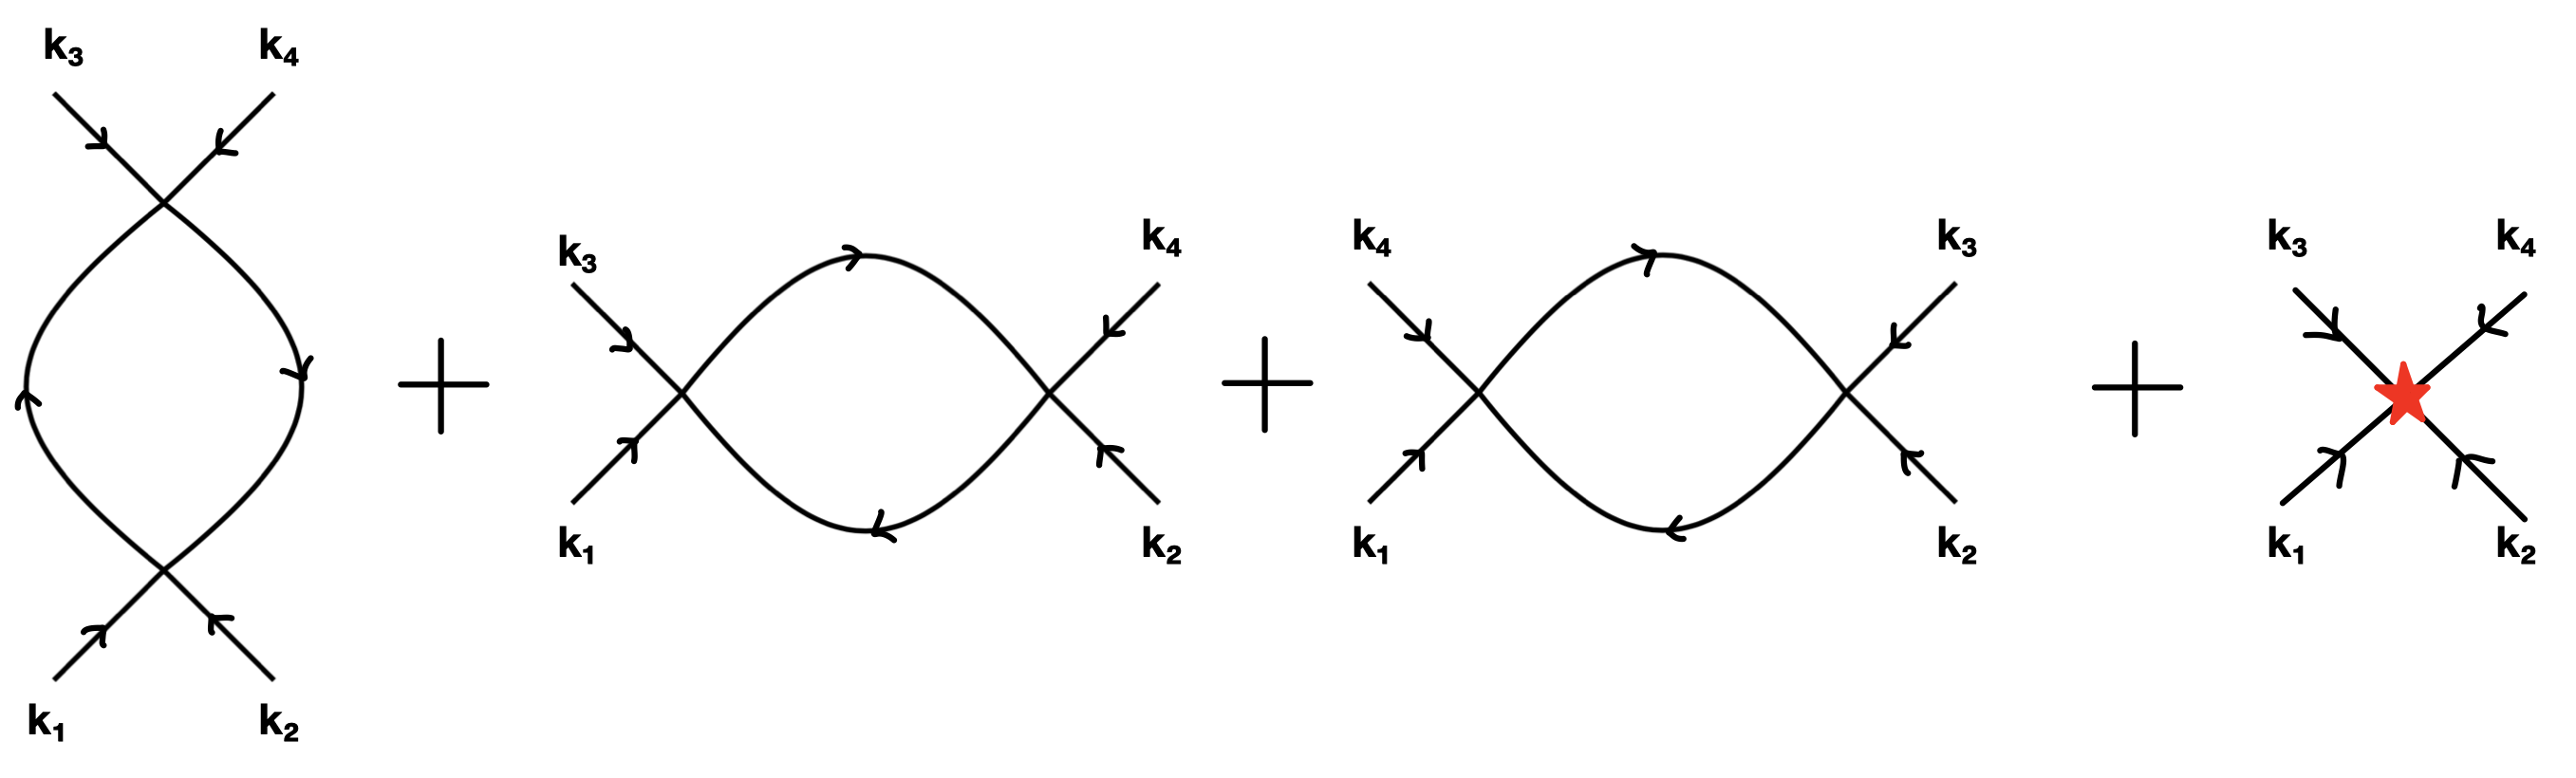
\includegraphics[align=c, width=0.6\linewidth]{pics/KG-4.png}\\
	&= \frac{g_R^2}{2} \left[iF(s)+iF(t)+iF(u)\right] -iCg_R,
\end{aligned}
\end{equation}
where we have introduced three momentum parameters $s$, $t$, and $u$: 
\begin{equation}
	s = (k_1+k_2)^2,\quad
	t = (k_1+k_3)^2,\quad
	u = (k_1+k_4)^2.
\end{equation}
The loop integrals for three channels are the same, denoted by
\begin{equation}
	iF(k^2) = \int \frac{d^4 q}{(2\pi)^4} \Delta_0(q) \Delta_0(q+k).
\end{equation}
The integral is again divergent.



\subsubsection{Regularization}
The denominator in the integral
\begin{equation}
	iF(k^2) = \int \frac{d^4 q}{(2\pi)^4} \frac{i}{q^2-m_R^2} \frac{i}{(q+k)^2-m_R^2}
\end{equation}
involves multiplication of two polynomial.
The expression can be simplified by the \textit{Feynman parametrization}, which is essentially the identity:
\begin{equation}
	\frac{1}{A_{1} \ldots A_{n}}=\int d F_{n}\left(x_{1} A_{1}+\ldots+x_{n} A_{n}\right)^{-n},
\end{equation}
where the integration measure over the Feynman parameters $x_{i}$ is
\begin{equation}
	\int d F_{n}=(n-1) ! \int_{0}^{1} d x_{1} \ldots d x_{n} \delta\left(x_{1}+\ldots+x_{n}-1\right).
\end{equation}
This measure is normalized so that $\int d F_{n} =1$. 
The simplest case is
\begin{equation}
	\frac{1}{A B}=\int_{0}^{1} \frac{dx}{[A+(B-A) x]^{2}}
	=\int_{0}^{1} \frac{\delta(x+y-1)}{[x A+y B]^{2}} dx dy.
\end{equation}
Other useful identities are
\begin{equation}
\begin{aligned}
	\frac{1}{A B^{n}} &=\int_{0}^{1} dxdy\frac{\delta(x+y-1)n y^{n-1}}{[x A+y B]^{n+1}} , \\
	\frac{1}{A B C} &=\int_{0}^{1} dxdydz \frac{2\delta(x+y+z-1)}{[x A+y B+z C]^{3}} .
\end{aligned}
\end{equation}

Using the Feynman parameters, the integral is
\begin{equation}
	iF(k^2) = \frac{i\Omega_4}{(2\pi)^4} \int_0^1 dx \int dq\ \frac{q^{3}}{\left[q^2+m_R^2+x(1-x)k^2\right]^2}.
\end{equation}
Using the dimensional regularization, the integral is
\begin{equation}
	iF_\varepsilon(k^2) = \frac{i\tilde{\mu}^{\varepsilon}\Omega_{4-\varepsilon}}{(2\pi)^{4-\varepsilon}} \int_0^1 dx \int dq\ \frac{q^{3-\varepsilon}}{\left[q^2+m_R^2+x(1-x)k^2\right]^2}.
\end{equation}
Then we carry out the calculation, the result is:
\begin{equation}
\begin{aligned}
	F_\varepsilon(s) &= \frac{1}{8\pi^2\varepsilon} + \frac{1}{16\pi^2}\int_0^1 dx \ln \left(\frac{4\pi \tilde{\mu}^2 e^{-\gamma_E}}{D_{s,x}}\right) \\
	&= \frac{1}{8\pi^2\varepsilon} +\frac{1}{8\pi^2}\ln \left(\frac{\mu}{m_R}\right) - \frac{1}{16\pi^2}\int_0^1 dx \ln\left(\frac{D_{s,x}}{m_R^2}\right),
\end{aligned}
\end{equation}
where we have denote
\begin{equation}
	D_{k^2,x} \equiv m_R^2+x(1-x)k^2.
\end{equation}
Now sum up the contribution from all channel, the result looks like:
\begin{equation}
	\Gamma^{(2)}_4 = \frac{3 g_R^2}{16\pi^2}\left[\frac{1}{\varepsilon} + \ln\left(\frac{\mu}{m_R}\right)\right] - \frac{g_R^2}{32\pi^2}\int_0^1 dx \ln\left(\frac{D_{s,x}D_{t,x}D_{u,x}}{m_R^6}\right)- C g_R.
\end{equation}


\subsubsection{Renormalization and Physical Observables}

To absorb the divergence, we can choose the counter term coefficient as
\begin{equation}
	C = \frac{3g_R}{16\pi^2}.
\end{equation}
So, to the second order, the vertex function is:
\begin{equation}
	\Gamma_4(k_1,k_2,k_3,k_4) = -g_R + \frac{g_R^2}{32\pi^2}\int_0^1 dx \ln\left(\frac{\mu^6}{D_{s,x}D_{t,x}D_{u,x}}\right).
\end{equation}
The vertex function is directly related to the physical observables.
It can be measured in the scattering experiment or just just by the repulsive force it generated.
We can choose the scale $\mu_0$ so that
\begin{equation}
	\Gamma(m_R,m_R,m_R,m_R) = -g_R.
\end{equation}
Then the corrected vertex function gives the physical predictions, for example on the scattering amplitude for different $k_i$'s.

\subsection{Renormalization Group}
Now consider the RG equation for the one-loop correction. 
The bare parameters are:
\begin{equation}
	g_0 = Z_g g\tilde{\mu}^{\epsilon},\ 
	m_0 = Z_m^{1/2} m,
\end{equation}
The RG conditions are:
\begin{eqnarray}
	\frac{d g_0}{d\ln \mu}
	&=& \left(\frac{3}{16\pi^2 \epsilon} + \frac{1}{g}\right)\frac{dg}{d\ln \mu} + \epsilon = 0, \\
	\frac{d m_0}{d\ln \mu}
	&=& \frac{1}{32\pi^2 \epsilon}\frac{dg}{d\ln \mu} + \frac{1}{m}\frac{dm}{d \ln \mu} = 0.
\end{eqnarray}
Consider the series expansion of beta function:
\begin{equation}
	\beta(g) = \frac{dg}{d\ln \mu} = \beta_1 g + \beta_2 g^2 +O(g^3).
\end{equation}
The beta function is
\begin{equation}
	\beta(g) = -\epsilon g + \frac{3g^2}{16\pi^2} + O(g^3).
\end{equation}
The anomalous dimension of mass is
\begin{equation}
	\gamma_m = \frac{1}{m}\frac{dm}{d \ln \mu} = \frac{g}{32\pi^2}+O(g^2)
\end{equation}

\section{Wilsonian Renormalization Group}
Now we consider the two-loop correction to the self energy
\begin{equation}
\begin{aligned}
	i\Sigma^{(2)}(k) 
	&= -\frac{g_R^2}{3!} \int \frac{d^4 p_1}{(2\pi)^4}\frac{d^4 p_2}{(2\pi)^4} \frac{i}{p_1^2-m_R^2} \frac{i}{p_2^2-m_R^2} \frac{i}{(k-p_1-p_2)^2-m_R^2} \\
	&= i\frac{g_R^2}{3!} \int \frac{d^4 p_1}{(2\pi)^4}\frac{d^4 p_2}{(2\pi)^4} \int_0^1 dx dy dz\  \frac{2 \delta(1-x-y-z) }{D_{x,y,z}^3},
\end{aligned}
\end{equation}
where the denominator is a bilinear
\begin{equation}
	D = \left(\begin{array}{cc} p_1 & p_2 \end{array} \right) 
		\left[\begin{array}{cc} x+z & z \\ z & y+z \end{array} \right]
		\left(\begin{array}{c} p_1 \\ p_2 \end{array} \right) 
		- 2kz (p_1 + p_2) + k^2z - m_R^2.
\end{equation}

For a generic bilinear, we can simplify it by shifting the variable and diagonalized the quadratic coefficient matrix (which is always symmetric):
\begin{equation}
\begin{aligned}
	D &= \sum_{ij} A_{ij} p_i p_j + \sum_i B_i p_i - C \\
	&= \sum_{ij} A_{ij}p'_i p'_j - C - \frac{1}{4} \sum_{ij} B_i A^{-1}_{ij} B_j \\
	&= \sum_n a_n p''_n p''_n - C',
\end{aligned}
\end{equation}
We do not really need to carry out the diagonalization explicitly, but the above general form tells tells us that the integral can be transformed to
\begin{equation}
\begin{aligned}
	\frac{1}{D_{x,y,z}^3} 
	&\rightarrow \frac{1}{(\det A)^2} \frac{1}{\left[p_1^2 + p_2^2 - C'\right]^3} \\
	&= \frac{1}{[xy+yz+zx]^2} \frac{1}{\left[ p_1^2+p_2^2 - \left(-\frac{xyz}{xy+yz+zx}k^2+m_R^2\right)\right]^3}
\end{aligned}
\end{equation}
The self energy is then
\begin{equation}
	\Sigma^{(2)}(k) = -\frac{g_R^2}{3!} \int_0^1 \frac{dF_3}{[xy+(x+y)z]^2} I(p_1^2,p_2^2), 
\end{equation}
where
\begin{equation}
	I_\varepsilon(p_1^2,p_2^2) = \frac{\tilde{\mu}^{2\varepsilon}\Omega_d^2}{(2\pi)^{2d}} \int dp_1 dp_2 \frac{p_1^{d-1} p_2^{d-2}}{(p_1^2+p_2^2+C')^3}
\end{equation}

\subsection{Regularization and Renormalization}
The $\varepsilon$ expansion gives:
\begin{equation}
	I_\varepsilon(p_1^2,p_2^2) = -\frac{C'}{512 \pi^4 \varepsilon} + \text{finite part}.
\end{equation}
Back to the 
\begin{equation}
	\frac{g_R^2}{3\cdot 2^{10} \pi^4 \varepsilon} \int_0^1 dF_3\ \frac{xyz}{(xy+yz+zx)^3} k^2
\end{equation}


\section{Spontaneously Symmetry Breaking}




